\documentclass{standalone}
\usepackage{pgfplots}
\pgfplotsset{compat=1.18}
\usepgfplotslibrary{colorbrewer}
\pgfplotsset{cycle list/Set1-6}

\begin{document}

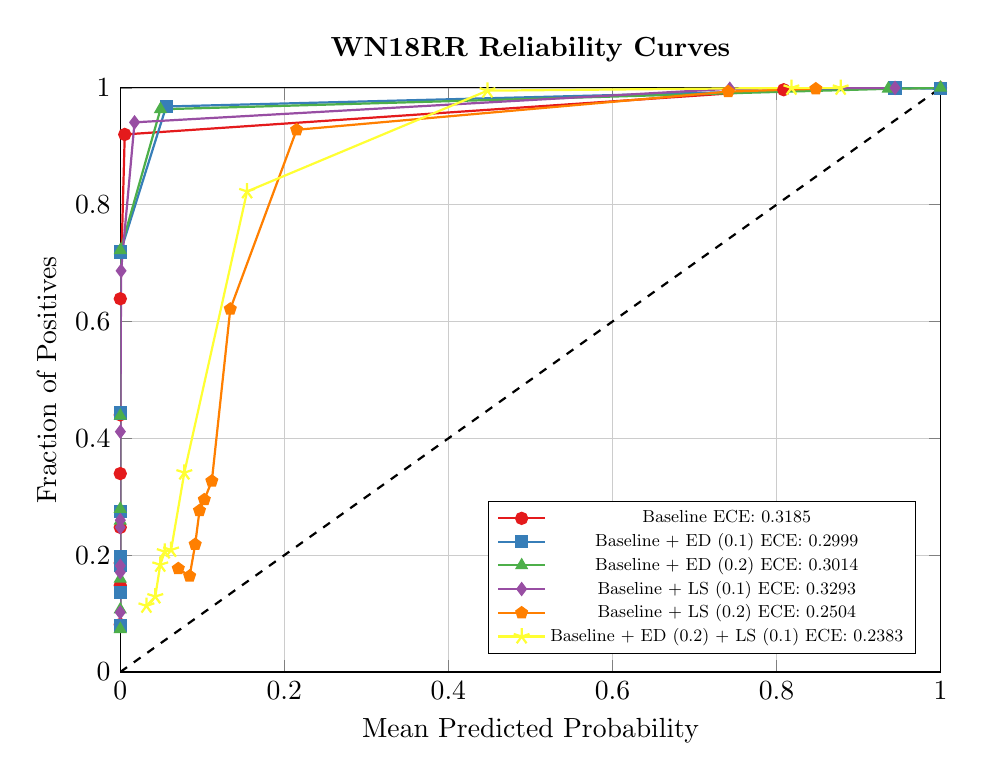
\begin{tikzpicture}
\begin{axis}[
    title={\textbf{WN18RR Reliability Curves}},
    xlabel={Mean Predicted Probability},
    ylabel={Fraction of Positives},
    xmin=0, xmax=1,
    ymin=0, ymax=1,
    xtick={0, 0.2, 0.4, 0.6, 0.8, 1.0},
    ytick={0, 0.2, 0.4, 0.6, 0.8, 1.0},
    legend pos=south east,
    legend style={nodes={scale=0.7, transform shape}, font=\small},
    grid=both,
    grid style={line width=.1pt, draw=gray!20},
    major grid style={line width=.2pt, draw=gray!40},
    width=12cm,
    height=9cm,
    cycle list name=Set1-6
]

% Perfectly Calibrated Line
\addplot [color=black, dashed, line width=0.8pt, forget plot]
    coordinates {(0,0)(1,1)};

% Model 1: Baseline
% File: wn18rr_baseline.txt 
\addplot+[mark=*, thick] coordinates {
    (5.26113353e-10, 0.08133971) (1.26847587e-08, 0.14832536) (9.62602527e-08, 0.18660287) (4.30059238e-07, 0.24760383)
    (1.82554167e-06, 0.33971292) (8.74549796e-06, 0.44019139) (8.05865042e-05, 0.63897764) (5.47991630e-03, 0.92025518)
    (8.08705782e-01, 0.99681021) (9.99806225e-01, 1.0)
};
\addlegendentry{Baseline ECE: 0.3185}

% Model 2: Baseline + ED (0.1)
% File: wn18rr_ed_0.1.txt 
\addplot+[mark=square*, thick] coordinates {
    (1.59377025e-13, 0.07974482) (3.38801914e-11, 0.13556619) (9.93519280e-10, 0.18341308) (1.48955417e-08, 0.19808307)
    (2.14946716e-07, 0.27432217) (3.77242807e-06, 0.44338118) (2.31945242e-04, 0.71884984) (5.60054895e-02, 0.96810207)
    (9.44394010e-01, 1.0) (9.99964201e-01, 0.9984051)
};
\addlegendentry{Baseline + ED (0.1) ECE: 0.2999}

% Model 3: Baseline + ED (0.2)
% File: wn18rr_ed_0.2.txt 
\addplot+[mark=triangle*, thick] coordinates {
    (2.40124033e-14, 0.07336523) (5.03503951e-12, 0.10685805) (1.68613258e-10, 0.15948963) (3.19757249e-09, 0.25878594)
    (4.92120305e-08, 0.27910686) (1.05490864e-06, 0.43859649) (1.46652632e-04, 0.72204473) (4.90035375e-02, 0.96331738)
    (9.36193196e-01, 0.9984051) (9.99954469e-01, 1.0)
};
\addlegendentry{Baseline + ED (0.2) ECE: 0.3014}

% Model 4: Baseline + LS (0.1)
% File: wn18rr_ls_0.1.txt 
\addplot+[mark=diamond*, thick] coordinates {
    (1.10222183e-06, 0.10207337) (4.58455482e-06, 0.17065391) (1.11118820e-05, 0.18181818) (2.41768720e-05, 0.24760383)
    (5.51292064e-05, 0.2599681) (1.63944675e-04, 0.41148325) (1.02250549e-03, 0.68690096) (1.74143657e-02, 0.94098884)
    (7.43007706e-01, 0.9984051) (9.44419871e-01, 1.0)
};
\addlegendentry{Baseline + LS (0.1) ECE: 0.3293}

% Model 5: Baseline + LS (0.2)
% File: wn18rr_ls_0.2.txt 
\addplot+[mark=pentagon*, thick] coordinates {
    (0.07075277, 0.17703349) (0.08458012, 0.16427432) (0.09133959, 0.2185008) (0.09661624, 0.27635783)
    (0.10248154, 0.29505582) (0.1116392, 0.32695375) (0.13413999, 0.62140575) (0.21502426, 0.92822967)
    (0.74106713, 0.99362041) (0.8478785, 0.9984051)
};
\addlegendentry{Baseline + LS (0.2) ECE: 0.2504}

% Model 6: Baseline + ED (0.2) + LS (0.1)
% File: wn18rr_combined.txt 
\addplot+[mark=star, thick, mark size=3pt] coordinates {
    (0.0318882, 0.11323764) (0.04268097, 0.1291866) (0.04875135, 0.18341308) (0.05421272, 0.20607029)
    (0.06196919, 0.20893142) (0.0781092, 0.34130781) (0.15462148, 0.82268371) (0.44764138, 0.99521531)
    (0.8181518, 1.0) (0.87820525, 1.0)
};
\addlegendentry{Baseline + ED (0.2) + LS (0.1) ECE: 0.2383}

\end{axis}
\end{tikzpicture}

\end{document}